\documentclass[a4paper]{article}
\usepackage[ngerman]{babel}
\usepackage{multicol}
\usepackage{calc}
\usepackage{ifthen}
\usepackage[landscape,left=1cm,top=1cm,right=1cm,nohead,nofoot]{geometry}
\usepackage{amsmath,amsthm,amsfonts,amssymb}
\usepackage{color,graphicx,overpic}
\usepackage{listings}
\usepackage[compact]{titlesec} %less space for headers
\usepackage{mdwlist} %less space for lists
\usepackage[utf8]{inputenc}
\usepackage{tikz}
\usepackage{pdflscape}
\usepackage{verbatim}
\usetikzlibrary{mindmap, arrows,shapes,positioning,shadows,trees}
\tikzstyle{every node}=[draw=black,thin,anchor=west, minimum height=2em]
\usepackage[hidelinks,pdfencoding=auto]{hyperref}

\pdfinfo{
    /Title (Automaten, Sprachen \& Komplexität - Cheatsheet)
    /Creator (TeX)
    /Producer (pdfTeX 1.40.0)
    /Author (Robert Jeutter)
    /Subject ()
}
% Information boxes
\newcommand*{\info}[4][16.3]{
  \node [ annotation, #3, scale=0.65, text width = #1em, inner sep = 2mm ] at (#2) {
  \list{$\bullet$}{\topsep=0pt\itemsep=0pt\parsep=0pt
    \parskip=0pt\labelwidth=8pt\leftmargin=8pt
    \itemindent=0pt\labelsep=2pt}
    #4
  \endlist
  };
}

% This sets page margins to .5 inch if using letter paper, and to 1cm
% if using A4 paper. (This probably isn't strictly necessary.)
% If using another size paper, use default 1cm margins.
\ifthenelse{\lengthtest { \paperwidth = 11in}}
    { \geometry{top=.5in,left=.5in,right=.5in,bottom=.5in} }
    {\ifthenelse{ \lengthtest{ \paperwidth = 297mm}}
        {\geometry{top=1cm,left=1cm,right=1cm,bottom=1cm} }
        {\geometry{top=1cm,left=1cm,right=1cm,bottom=1cm} }
    }

% Redefine section commands to use less space
\makeatletter
\renewcommand{\section}{\@startsection{section}{1}{0mm}%
                                {-1ex plus -.5ex minus -.2ex}%
                                {0.5ex plus .2ex}%x
                                {\normalfont\large\bfseries}}
\renewcommand{\subsection}{\@startsection{subsection}{2}{0mm}%
                                {-1explus -.5ex minus -.2ex}%
                                {0.5ex plus .2ex}%
                                {\normalfont\normalsize\bfseries}}
\renewcommand{\subsubsection}{\@startsection{subsubsection}{3}{0mm}%
                                {-1ex plus -.5ex minus -.2ex}%
                                {1ex plus .2ex}%
                                {\normalfont\small\bfseries}}
\makeatother

% Define BibTeX command
\def\BibTeX{{\rm B\kern-.05em{\sc i\kern-.025em b}\kern-.08em
    T\kern-.1667em\lower.7ex\hbox{E}\kern-.125emX}}

% Don't print section numbers
\setcounter{secnumdepth}{0}

\setlength{\parindent}{0pt}
\setlength{\parskip}{0pt plus 0.5ex}    
% compress space
\setlength\abovedisplayskip{0pt}
\setlength{\parskip}{0pt}
\setlength{\parsep}{0pt}
\setlength{\topskip}{0pt}
\setlength{\topsep}{0pt}
\setlength{\partopsep}{0pt}
\linespread{0.5}
\titlespacing{\section}{0pt}{*0}{*0}
\titlespacing{\subsection}{0pt}{*0}{*0}
\titlespacing{\subsubsection}{0pt}{*0}{*0}

%My Environments
\newtheorem{example}[section]{Example}

% Turn off header and footer
\pagestyle{empty}
\begin{document}

\begin{tikzpicture}[
        topic/.style={
                text centered,
                text width=6cm,
                level distance=1mm,
                sibling distance=5mm,
                rounded corners=2pt
            },
        subtopic/.style={
                yshift=1.5cm,
                text centered,
                text width=3cm,
                rounded corners=2pt,
                fill=gray!10
            },
        theme/.style={
                grow=down,
                xshift=-0.6cm,
                text centered,
                text width=5cm,
                edge from parent path={(\tikzparentnode.205) |- (\tikzchildnode.west)}
            },
        description/.style={
                grow=down,
                xshift=-2cm,
                text width=7cm,
                right,
                text centered,
                edge from parent path={(\tikzparentnode.189) |- (\tikzchildnode.west)}
            },
        level 1/.style={sibling distance=9cm},
        level 1/.append style={level distance=2.5cm},
    ]
    %topic
    \node[topic]{Grundbegriffe}
    child{node [subtopic]{Wort}
            child[theme, level distance=1cm] { node { Präfix}
                    child[description, level distance=1cm]{node {wenn es $z\in\sum^*$ gibt mit $yz=w$}}
                }
            child[theme, level distance=3cm] { node { Infix/Faktor }
                    child[description, level distance=1cm]{node {wenn es $x,z\in\sum^*$ gibt mit $xyz = w$}}
                }
            child[theme, level distance=5cm] { node { Suffix}
                    child[description, level distance=1cm]{node {wenn es $x\in\sum^*$ gibt mit $xy=w$}}
                }
        }
    child{node [subtopic]{Sprache}
            child [theme, level distance=1cm] { node {Chomsky Hierachie}
                    child[description, level distance=1cm] { node {Typ 0: Allgemein \\ jede Grammatik ist vom Typ 0}}
                    child[description, level distance=2.5cm] { node {Typ 1: Kontextsensitiv \\ wenn es Wörter $u,v,w\in(V\cup\sum)^*,|v|>0$ und ein Nichtterminal $A\in V$ gibt mit $l=uAw$ und $r=uvw$}}
                    child[description, level distance=4cm] { node {Typ 2: Kontextfrei \\ wenn $l\in V$ und $r\in (V\cup \sum)^*$ gilt}}
                    child[description, level distance=5.2cm] { node {Typ 3: Regulär \\ wenn $l\in V$ und $r\in \sum V\cup {\epsilon}$ gilt}}
                }
            child[theme, level distance=7.4cm]{node {Kleene Abschluss $L*=\bigcup_{n\geq 0} L^n$}
                    %child[description, level distance=1cm]{node{$L*=\bigcup_{n\geq 0} L^n$}}
                }
        }
    child{node [subtopic]{Grammatik}
            child[theme, level distance=1cm] { node {Symbole}
                    child[description, level distance=1cm] { node {Nicht-Terminale, Großbuchstaben, Elemente aus V}}
                    child[description, level distance=2cm] { node {Terminale, Kleinbuchstaben, Elemente aus $\sum$}}
                }
            child[theme, level distance=4cm]{ node {4-Tupel $G=(V,\sum, P, S)$}
                    child[description, level distance=1cm] { node {V ist eine endliche Menge von Nicht-Terminalen oder Variablen}}
                    child[description, level distance=2cm] { node {$\sum$ ist Alphabet (Menge der Terminale)}}
                    child[description, level distance=3cm] { node {$P$ ist eine endliche Menge von Regeln oder Produktionen}}
                    child[description, level distance=4cm] { node {$S\in V$ ist das Startsymbol oder das Axiom}}
                }
        };
\end{tikzpicture}

\begin{tikzpicture}[
        topic/.style={
                text centered,
                text width=6cm,
                level distance=1mm,
                sibling distance=5mm,
                rounded corners=2pt
            },
        subtopic/.style={
                yshift=1.5cm,
                text centered,
                text width=3cm,
                rounded corners=2pt,
                fill=gray!10
            },
        theme/.style={
                grow=down,
                xshift=-0.6cm,
                text centered,
                text width=5cm,
                edge from parent path={(\tikzparentnode.205) |- (\tikzchildnode.west)}
            },
        description/.style={
                grow=down,
                xshift=-2cm,
                text width=5cm,
                right,
                text centered,
                edge from parent path={(\tikzparentnode.189) |- (\tikzchildnode.west)}
            },
        level 1/.style={sibling distance=7cm},
        level 1/.append style={level distance=2.5cm},
    ]
    % Topic
    \node[topic]{intuitiv (loop) berechenbar}
    child{node [subtopic]{$\mu$ rekurisv}
            child[theme, level distance=1cm]{node{Definition}
                    child[description, level distance=1cm]{node{$\mu f:\mathbb{N}^k\rightarrow\mathbb{N}$ definiert durch }}
                    child[description, level distance=2cm]{node{$\mu f(n_1,...,n_k)= min\{m| f(m,n_1,...,n_k)=0$ und }}
                    child[description, level distance=3cm]{node{$\forall x< m: f(x,n_1,...,n_k) \text{ definiert } \}$.}}
                }
        }
    child{node [subtopic]{while berechnenbar}
            child[theme, level distance=1cm]{node{Definition}
                    child[description, level distance=1.2cm]{node{$x_i=c; x_i=x_j+c; x_i=x_j-c$ mit $c\in\{0,1\}$ und $i,j\geq 1$ (Wertzuweisung) oder }}
                    child[description, level distance=2.5cm]{node{$P_1;P_2$, wobei $P_1$ und $P_2$ bereits While Programme sind oder }}
                    child[description, level distance=4cm]{node{while $x_i\not = 0$ do P end, wobei P ein While Programm ist und $i\geq 1$. }}
                }
            child[theme, level distance=6.5cm]{node {Gödel Vermutung}}
        }
    child{node [subtopic]{goto berechnenbar}
            child[theme, level distance=1cm]{node{endliche nichtleere File $P=A_1;A_2;...;A_m$ von Anweisungen $A_i$ der Form}
                    child[description, level distance=1.5cm]{node{$x_i=c, x_i=x_j+c, x_i=x_j-c$ mit $c\in\{0,1\}$ und $i,j\geq 1$}}
                    child[description, level distance=3cm]{node{goto l mit $0\leq l\leq m$ (unbedingter Sprung)}}
                    child[description, level distance=4.5cm]{node{if $x_i=0$ then l mit $i\geq 1$ und $0\leq l \leq m$ (bedingter Sprung)}}
                }
        }
    child{node [subtopic]{Turing berechenbar}
            child[theme, level distance=1cm]{node{Berechnung}
                    child[description, level distance=1cm]{node{Eingabe $x$ ist anfänglicher Bandinhalt}}
                    child[description, level distance=2.2cm]{node{Ausgabe $f(x)$ ist Bandinhalt (ohne Blanks am Rand)beim Erreichen eines Endzustands}}
                    child[description, level distance=3.6cm]{node{Hält die TM für die gegebene Eingabe nicht an, ist $f(x)$ an dieser Stelle undefiniert.}}
                }
            child[theme, level distance=5.8cm]{node{Church-Turing-These}
                    child[description, level distance=1.2cm]{node{Alle im intuitiven Sinne berechenbaren Funktionen können mit Turingmaschinen berechnet werden.}}
                }
        };
\end{tikzpicture}


\begin{tikzpicture}[
        topic/.style={
                text centered,
                text width=6cm,
                level distance=1mm,
                sibling distance=5mm,
                rounded corners=2pt
            },
        subtopic/.style={
                yshift=1.5cm,
                text centered,
                text width=5cm,
                rounded corners=2pt,
                fill=gray!10
            },
        theme/.style={
                grow=down,
                xshift=-1.6cm,
                text centered,
                text width=5cm,
                edge from parent path={(\tikzparentnode.192) |- (\tikzchildnode.west)}
            },
        description/.style={
                grow=down,
                xshift=-2cm,
                text width=5.3cm,
                right,
                text centered,
                edge from parent path={(\tikzparentnode.189) |- (\tikzchildnode.west)}
            },
        level 1/.style={sibling distance=7cm},
        level 1/.append style={level distance=2.5cm},
    ]
    \node[topic]{Rechtslineare Sprachen}
    child{node [subtopic] {endliche Automaten (Maschinen)}
    child[theme, level distance=1cm]{node{DFA $M$}
    child[description, level distance=1.2cm]{node{von einem DFA akzeptierte Sprache ist: $L(M)={w\in\sum^* | \hat{\delta}(z_0,w)\in E}$}}
    child[description, level distance=2.6cm]{node{Eine Sprache $L \supseteq \sum^*$ ist regulär, wenn es einen DFA mit $L(M)=L$ gibt}}
    }
    child[theme, level distance=4.8cm]{node{NFA $M$}
            child[description, level distance=1cm]{node {Jede von einem NFA akzeptierte Sprache ist regulär}}
        }
    child[theme, level distance=7cm]{node{Satz}
            child[description, level distance=1cm]{node {Wenn $L_1$ und $L_2$ reguläre Sprachen sind, dann ist auch}}
            child[description, level distance=2cm]{node { $L_1 \cup L_2$ regulär}}
            child[description, level distance=3cm]{node {$L_1 \cap L_2$ regulär}}
            child[description, level distance=4cm]{node {$L_1L_2$ regulär}}
            child[description, level distance=5cm]{node {$L_1^+/L_1^*$ regulär}}
        }
    child[theme, level distance=13cm]{node{ Jede reguläre Sprache ist rechtslinear}}
    }
    child{node [subtopic] {Reguläre Ausdrücke}
            child[theme, level distance=1cm]{node {Definition}
                    child[description, level distance=1.4cm]{node {Die Menge $Reg(\sum)$ der regulären Ausdrücke über dem Alphabet $\sum$ ist die kleinste Menge mit folgenden Eigenschaften:}}
                    child[description, level distance=2.9cm]{node {$\varnothing \in Reg(\sum), \lambda \in Reg(\sum), \sum \subseteq Reg(\sum)$}}
                    child[description, level distance=4cm]{node {Wenn $\alpha, \beta \in Reg(\sum)$, dann auch $(\alpha * \beta), (\alpha + \beta), (\alpha^*)\in Reg(\sum)$}}
                    child[description, level distance=5cm]{node {für $\alpha * \beta$ schreibt man oft $\alpha\beta$}}
                    child[description, level distance=6cm]{node {für $\alpha + \beta$ schreibt man auch $\alpha|\beta$}}
                }
            child[theme, level distance=8.5cm]{node {Für einen regulären Ausdruck $\alpha \in Reg(\sum)$ ist die Sprache $L(\alpha)\subseteq \sum^*$ induktiv definiert}
                    child[description, level distance=1.5cm]{node {zu jedem regulären Ausdruck $\gamma$ gibt es einen NFA M mit $L(\gamma)=L(M)$}}
                    child[description, level distance=3cm]{node {zu jedem DFA M gibt es einen regulären Ausdruck $\gamma$ mit $L(M)=L(\gamma)$}}
                }
        }
    child{node [subtopic] {Nicht-Reguläre Sprachen}
            child[theme, level distance=1cm]{node{ Pumping Lemma}
                    child[description, level distance=1.5cm]{node {L sei reguläre Sprache, dann gibt es $n\leq 1$ derart, dass für alle $x\in L$ mit $|x|\geq n$ gilt: es gibt Wörter $u,v,w \in \sum^*$ mit}}
                    child[description, level distance=3cm]{node {$x=uvw$, $|uv|\leq n$, $|v|\geq 1$}}
                    child[description, level distance=4cm]{node {$uv^i w\in L$ für alle $i\geq 0$}}
                    child[description, level distance=5cm]{node {geeignet um Aussagen über Nicht-Regularität zu machen}}
                }
            child[theme, level distance=7cm]{node{ Myhill-Nerode Äquivalenz}
                    child[description, level distance=1cm]{node {binäre Relation $R_L \subseteq \sum^* \times \sum^*$}}
                    child[description, level distance=2.3cm]{node {$\forall x,y\in \sum^*$ setze $(x,y)\in R_L$ genau dann, wenn $\forall z \in \sum^* :(xy\in L \leftrightarrow yz \in L)$ gilt. $x R_L y$}}
                    child[description, level distance=4cm]{node {Für Sprache L und Wort $x\in \sum^*$ ist $[x]_L=\{y\in\sum^* | x R_L y \}$ die Äquivalenzklasse von x}}
                    child[description, level distance=5.5cm]{node {Satz: L ist regulär $\leftrightarrow index(R_L)< \infty$}}
                }
        }
    child{node [subtopic] {Entscheidbarkeit}
            child[theme, level distance=1cm]{node{Wortproblem}
                    child[description, level distance=1cm]{node {Gilt $w\in L$ für eine gegebene reguläre Sprache L und $w\in\sum^*$?}}
                }
            child[theme, level distance=3cm]{node{Leerheitsproblem}
                    child[description, level distance=1cm]{node {Gilt $L=\varnothing$ für eine gegebene reguläre Sprache L?}}
                }
            child[theme, level distance=5cm]{node{Endlichkeitsproblem}
                    child[description, level distance=1cm]{node {Ist eine gegebene reguläre Sprache L endlich?}}
                }
            child[theme, level distance=7cm]{node{Schnittproblem}
                    child[description, level distance=1cm]{node {Gilt $L_1\cap L_2=\varnothing$ für gegebene reguläre $L_1,L_2$?}}
                }
            child[theme, level distance=9cm]{node{Inklusionsproblem}
                    child[description, level distance=1cm]{node {Gilt $L_1 \subseteq L_2$ für gegebene reguläre $L_1,L_2$?}}
                }
            child[theme, level distance=11cm]{node{Äquivalenzproblem}
                    child[description, level distance=1cm]{node {Gilt $L_1=L_2$ für gegebene reguläre $L_1,L_2$?}}
                }
        };
\end{tikzpicture}

\newpage
\begin{multicols*}{3}
    \paragraph{deterministischer endlicher Automat M}
    \begin{itemize*}
        \item 5-Tupel $M=(Z, \sum, z_0, \delta, E)$
        \item $Z$ eine endliche Menge von Zuständen
        \item $\sum$ das Eingabealphabet (mit $Z\cap\sum = \emptyset$)
        \item $z_0\in Z$ der Startzustand
        \item $\delta: Z \times \sum \rightarrow Z$ die Übergangsfunktion
        \item $E\subseteq Z$ die Menge der Endzustände
        \item kurz: DFA (deterministic finite automaton)
    \end{itemize*}

    \section{Turingmaschine (TM)}
    \begin{itemize*}
        \item 7-Tupel $M=(Z,\sum, \Phi, \delta, z_o, \Box, E)$
        \item $\sum$ das Eingabealphabet
        \item $\Phi$ mit $\Phi\supseteq\sum$ und $\Phi\cap Z\not= 0$ das Arbeits- oder Bandalphabet,
        \item $z_0\in Z$ der Startzustand,
        \item $\delta:Z\times\Phi\rightarrow(Z\times\Phi\times\{L,N,R\})$ die Überführungsfunktion
        \item $\Box\in\Phi/\sum$ das Leerzeichen oder Blank und
        \item $E\subseteq Z$ die Menge der Endzustände ist
    \end{itemize*}

    \section{Linksableitung}
    Eine Ableitung $S=w_0\Rightarrow ...\Rightarrow w_n = w\in\sum^*$ heißt Linksableitung, wenn in jedem Schritt das am weitesten links stehende Nichtterminal ersetzt wird (analog Rechtsabl.)

    \section{CYK-Algorithmus}
    Gehört ein gegebenes Wort zu $L(G)$?
    \begin{center}
        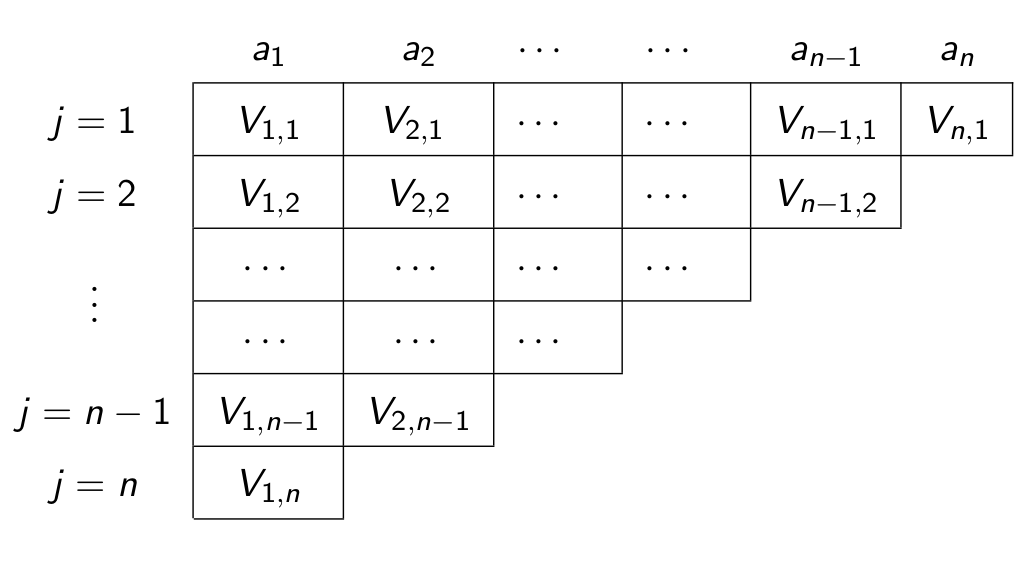
\includegraphics[width=\textwidth/4]{Assets/ASK_cyk-Algorithmus.png}
    \end{center}
    Von oben nach unten, von links unten nach rechts oben

    \section{Kellerautomaten}
    Um ein Automatenmodell für Kontextfreie Sprachen zu erhalten führt man einen Keller-(Pushdown)-Speicher ein, auf dem sich eine beliebig lange Sequenz von Zeichen befinden darf. Beim Einlesen eines neuen Zeichens wird das oberste Zeichen des Kellers gelesen und durch eine (evtl. leere) Sequenz von Zeichen ersetzt. An anderen Stellen kann der Keller nicht gelesen/geändert werden

    \columnbreak
    \section{Greibach-Normalform}
    Eine kontextfreie Grammatik G ist in Greibach Normalform falls alle Produktionen aus P folgende Form haben: $A\rightarrow aB_1B_2...B_k$, mit $k\in \mathbb{N}, A,B_1,...,B_k\in V$ und $a\in \sum$. Die Greibach Normalform garantiert, dass bei jedem Ableitungsschritt genau ein Alphabetsymbol entsteht.

    \section{Lemma von Ogden (William Ogden)}
    Wenn L eine kontextfreie Sprache ist, dann gibt es $n\geq 1$ derart, dass für alle $z\in L$, in denen $n$ Positionen markiert sind, gilt: es gibt Wörter $u,v,w,x,y\in\sum^*$ mit
    \begin{enumerate*}
        \item $z=uvwxy$
        \item v oder x enthält wenigstens eine der Markierungen oder
        \item $uv^i wx^i y \in L$ für alle $i\geq 0$
    \end{enumerate*}

    \section{Halteproblem}
    allgemein: Das Halteproblem ist die Menge aller Paare $(M,x)$,wobei $M$ eine TM ist und $x\in\{0,1\}^*$, sodass $M$ bei Eingabe von $x$ hält.

    \section{Reduktion}
    Seien $A\subseteq\sum^*,B\subseteq\Phi^*$. Eine Reduktion von A auf B ist eine totale und berechenbare Funktion $f:\sum^*\rightarrow\Phi^*$, so dass für alle $w\in\sum^*$ gilt: $w\in A\leftrightarrow f(x)\in B$. A heißt auf B reduzierbar (in Zeichen $A\leq B$), falls es eine Reduktion von A auf B gibt.

    \section{Satz von Rice}
    Sei $R$ die Klasse aller Turing-berechenbaren Funktionen $\{0,1\}^*\rightarrow\{0,1\}^*$, $\Omega$ die nirgendwo definierte Funktion und sei $S\subseteq \mathbb{R}$ mit $\Omega\in S$ und $\not = \mathbb{R}$. Dann ist die Sprache $C(S)=\{w\in L_{TM} | \phi_w\in S\}$ unentscheidbar.

    \section{Semi Entscheidbarkeit}
    Auch wenn das Halteproblem bei leerer Eingabe $H_0$ unentscheidbar ist, so kann doch nach endlicher Zeit festgestellt werden, daß die Maschine $M_w$ bei leerer Eingabe anhält - $H_0$ ist also ,,halb-'' oder ,,semi-entscheidbar''.

    Eine Sprache $L\subseteq \sum^*$ heißt semi-entscheidbar, falls die ,,halbe'' charakteristische Funktion von L, d.h. die partielle Funktion $X'_L:\sum^*\rightarrow \{1\}$ mit $x'_L=\begin{cases} 1 \quad\text{ falls } w\in L\\ undef. \quad\text{ falls } w\not\in L \end{cases}$ berechenbar ist.

    \columnbreak
    \section{Universelle Turing Maschine}
    eine Turing-Maschine, die jede Turing-Maschine simulieren kann, wenn deren Kodierung gegeben ist.
    Buchstaben des Bandalphabets als Wörter über $\{0, 1, 2\}$ mit $\Box = 2$ kodiert. Ab jetzt nehmen wir an, daß wir immer dieses Bandalphabet haben.

    Eine Turing Maschine U heißt universelle Turing Maschine, wenn sie die folgende partielle Funktion berechnet. $\{0,1\}^*\rightarrow\{0,1\}^*$
    $$y\rightarrow\begin{cases} \phi_w(x) \quad\text{ falls } y=w000x,w\in L_{TM},x\in\{0,1\}^* \\ undef. \quad\text{ sonst}\end{cases}$$

    \section{Totale berechenbare Funktionen}
    Gesucht ist $C\subseteq TOT \subseteq L_{TM}$, so dass $\{ \phi_w | w\in C \} = \{\phi_w | w \in TOT\}$ die Menge der totalen berechenbaren Funktionen ist.
    \begin{itemize*}
        \item $TOT$ ist nicht einmal semi-entscheidbar
        \item indirekt nehmen wir an, dass C semi-entscheidbar ist
        \item dann existiert eine totale berechenbare Funktion $f:\{0,1\}^*\rightarrow\{0,1\}^*$ mit Bild C
        \item neue Funktion $g:\{0,1\}^*\rightarrow\{0,1\}^*:w\vdash 1\phi_{f(w)}(w)$
    \end{itemize*}

    \section{Chomsky Normalform}
    Eine kontextfreie Grammatik G ist in Chomsky Normalform, falls alle Produktionen
    \begin{itemize}
        \item die Form $A\rightarrow AB$ oder $A\rightarrow a$ haben,
        \item und $S\rightarrow\epsilon$ und S nie auf der rechten Seite einer Produktion vorkommt
    \end{itemize}

\end{multicols*}
\end{document}
